\chapter{BTP Header Indication and Request} \label{app:BTPHeaderIndicationRequest}

\begin{figure}[htb]
	\centering
	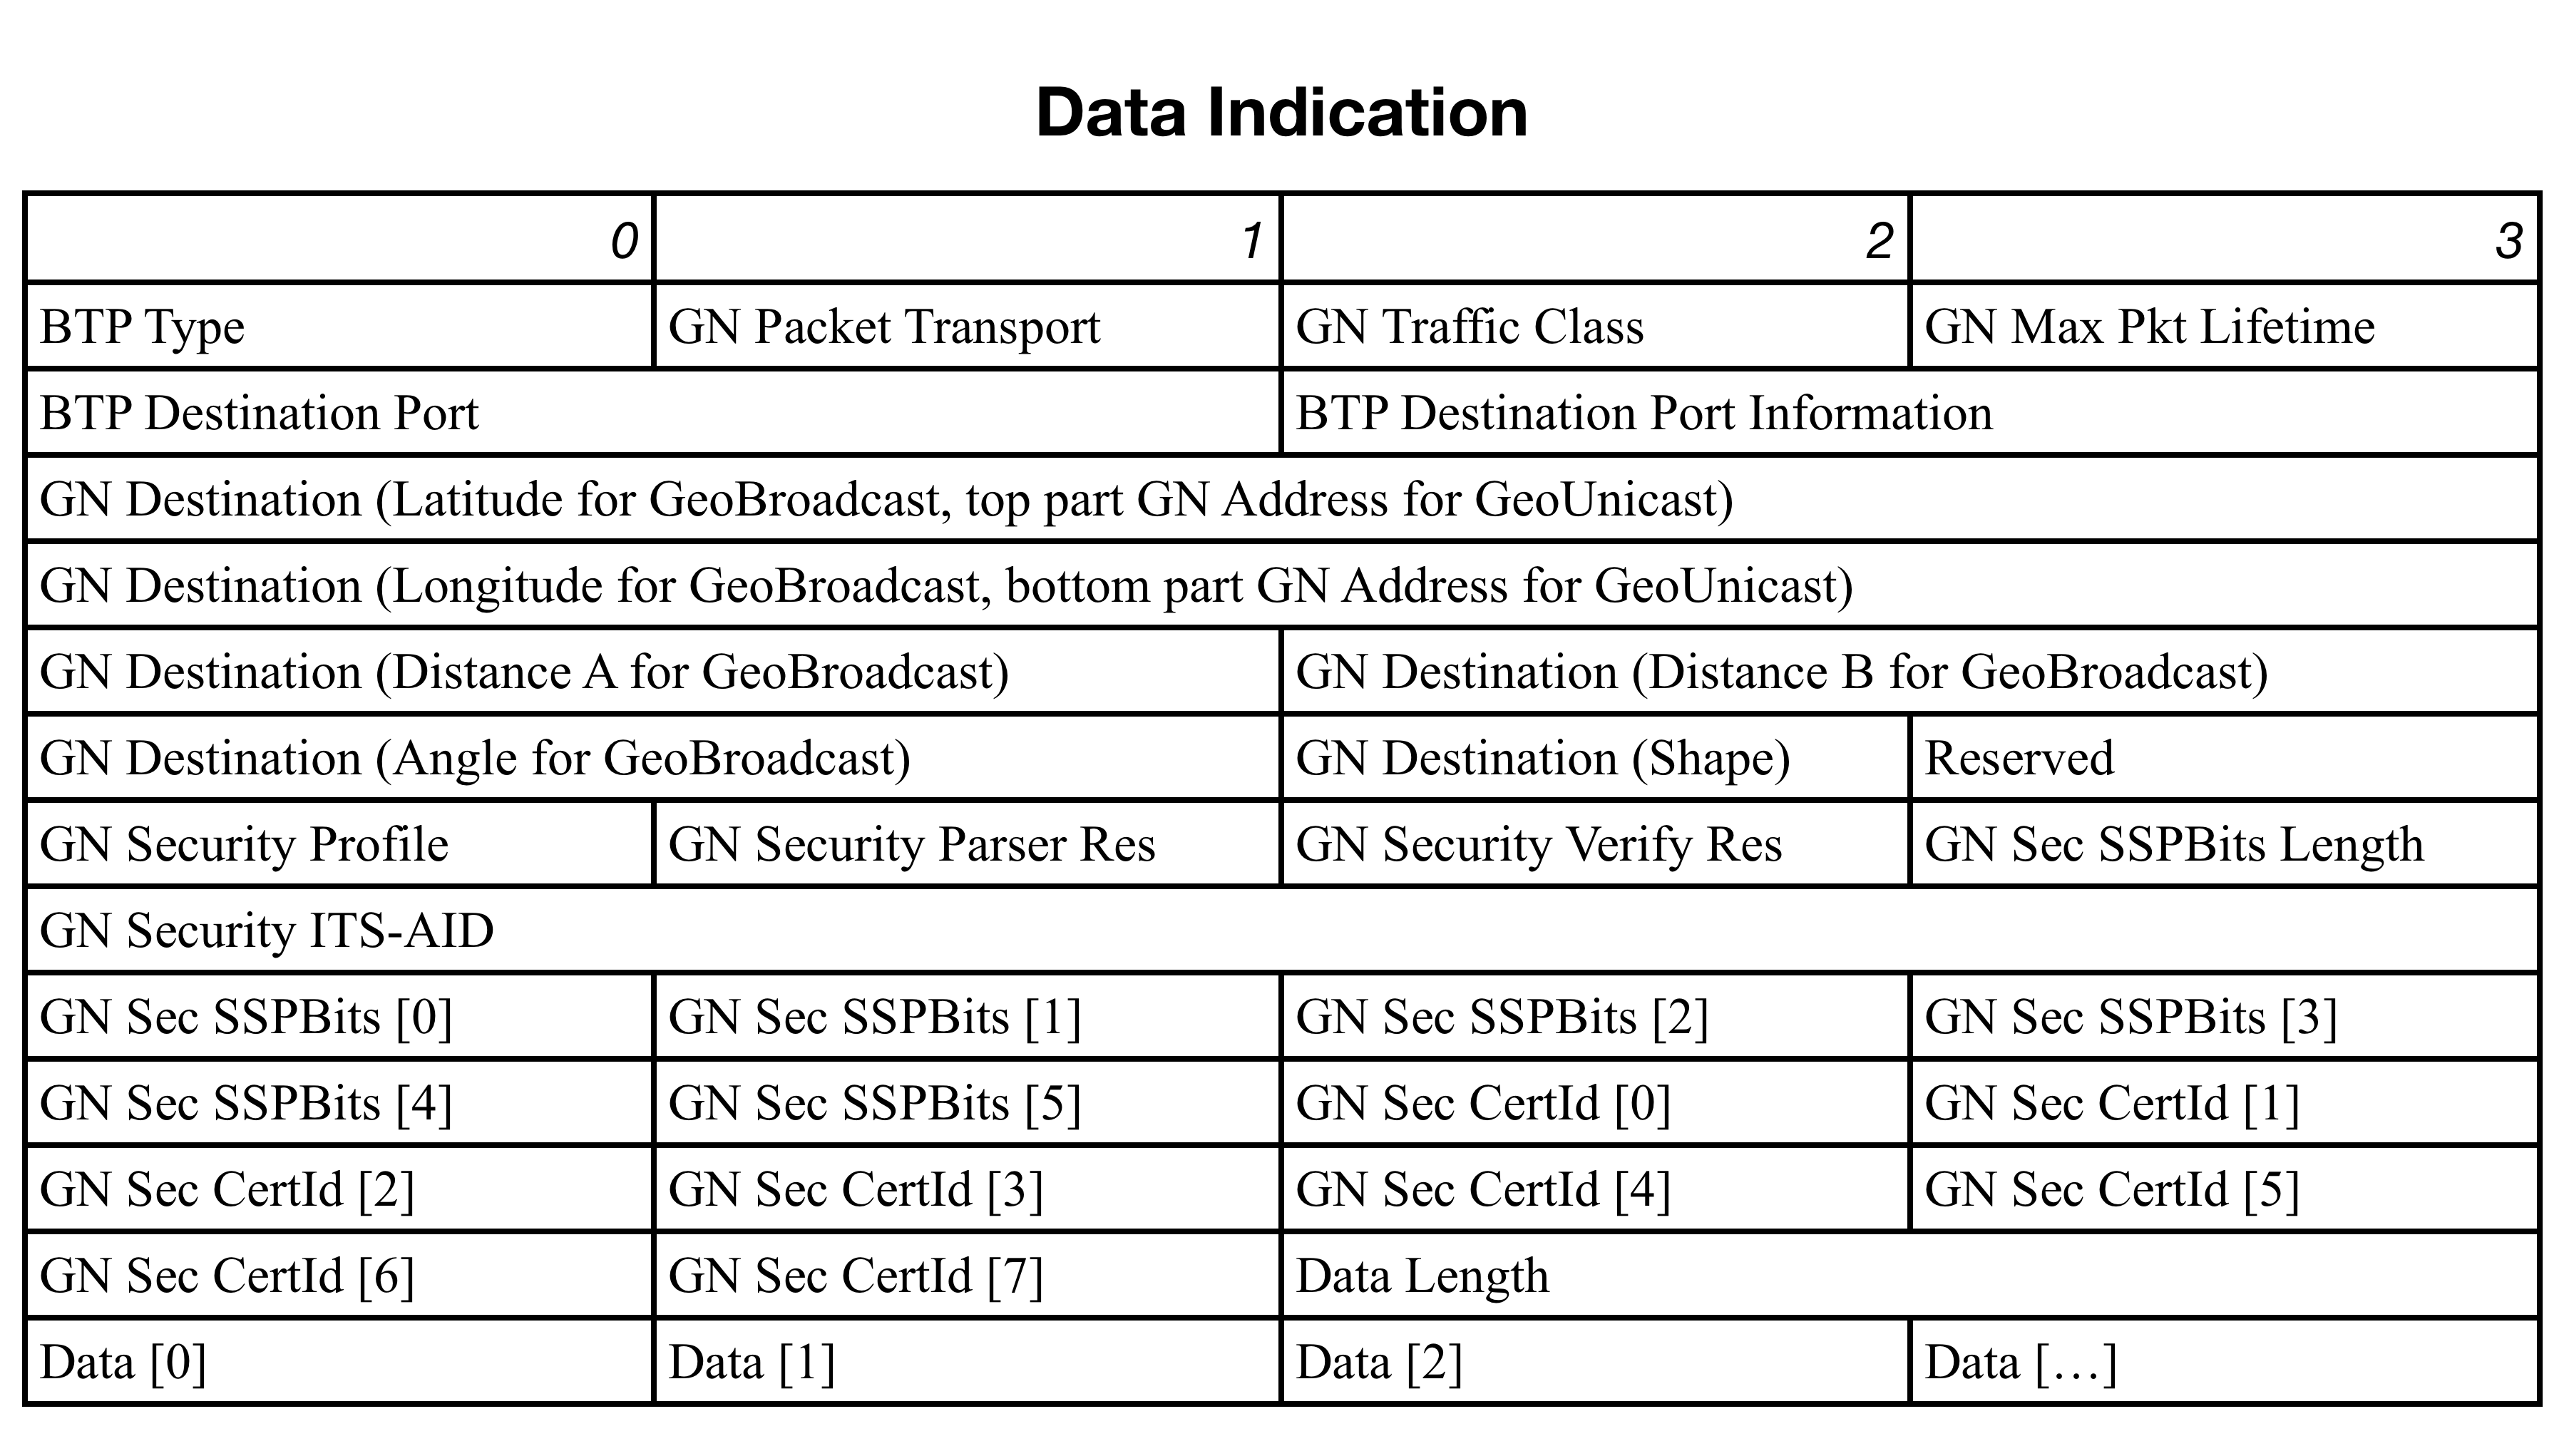
\includegraphics[width=1\textwidth]{images/BTPHeaderIndication}
	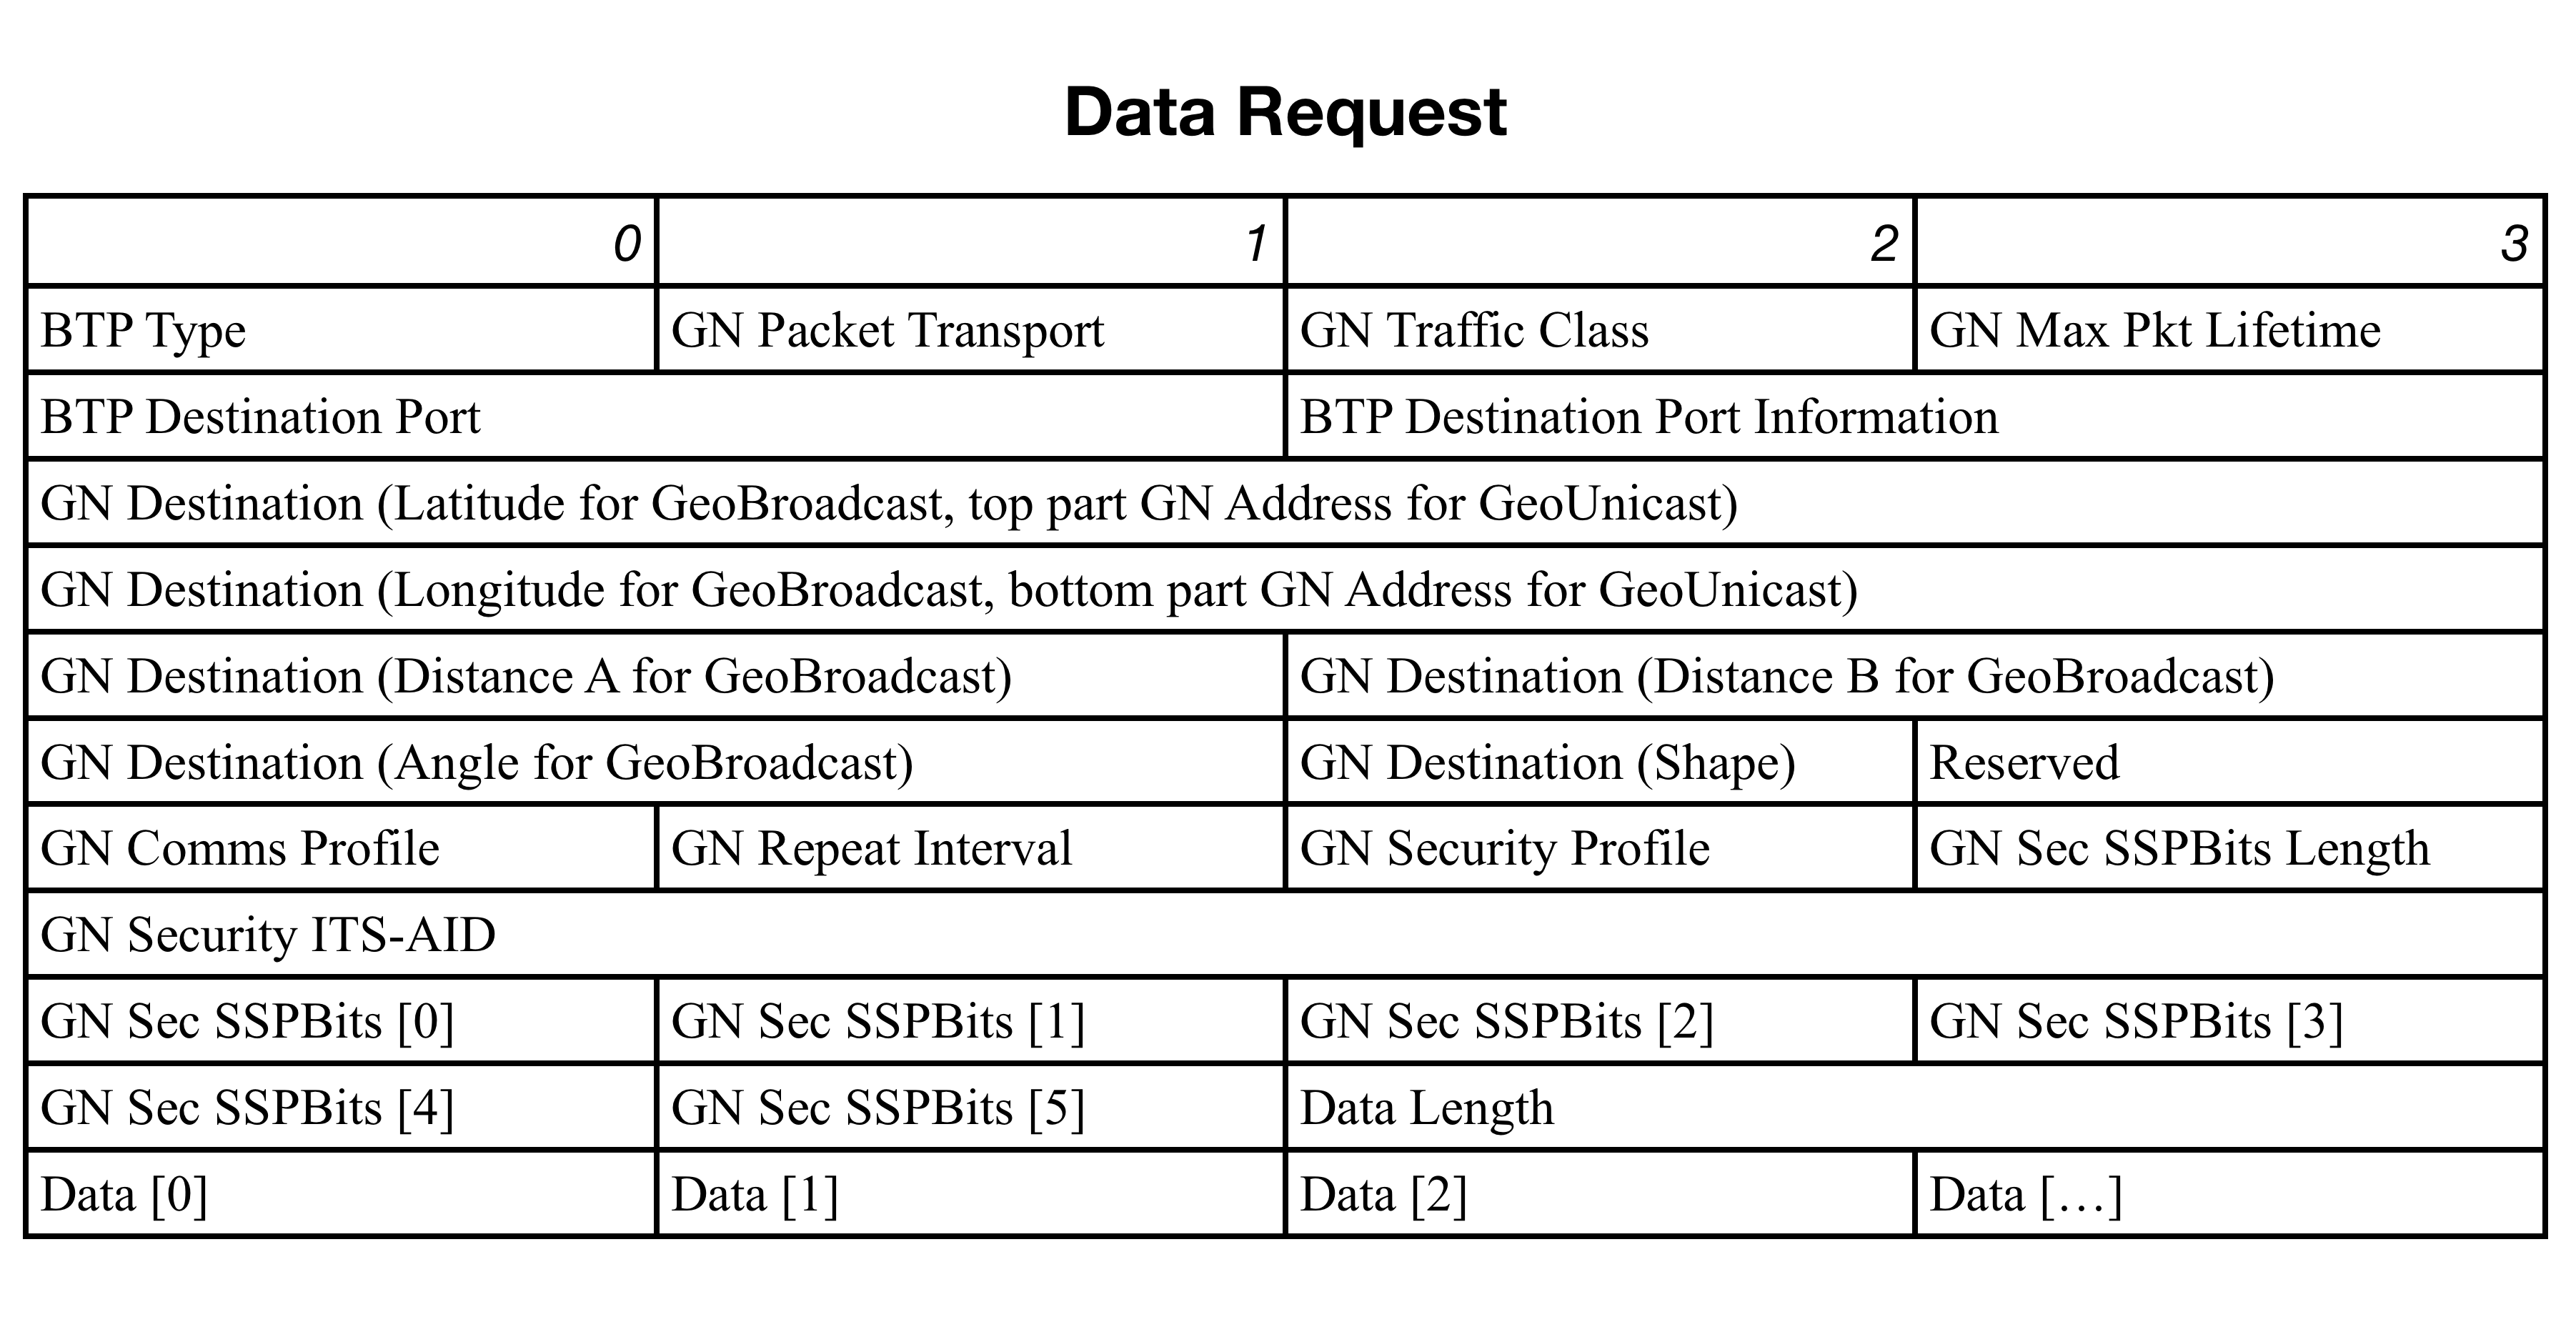
\includegraphics[width=1\textwidth]{images/BTPHeaderRequest}
	\caption{BTP Header}
	\label{fig:BTP_Indication}
	\cite{CohdaWirelessETSA}
\end{figure}

\clearpage
\newpage

\chapter{Measurements}
\section{GNSS Measurements}
\begin{figure}[htb]
	\centering
	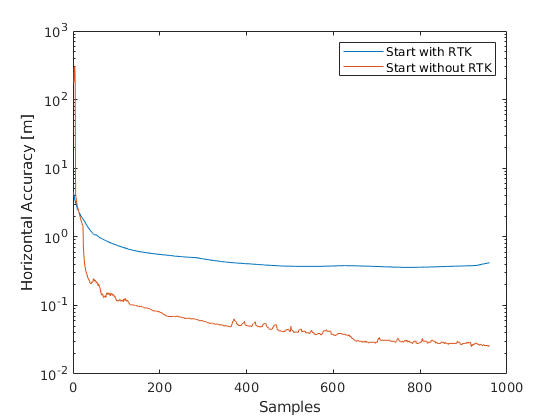
\includegraphics[width=0.6\textwidth]{images/AccuracyStart}
	\caption{The Horizontal Accuracy (PACC H) during a Start Up with RTK and without.}
	\label{fig:AccSt}
\end{figure}

In the figure\ref{fig:AccSt} the GNSS module is started and tries to get a fix. The measurement is done at the charging station, where the drift is big. The measurement was done about 3\;min with a rate of 5\;Hz.

\begin{figure}[htb]
	\centering
	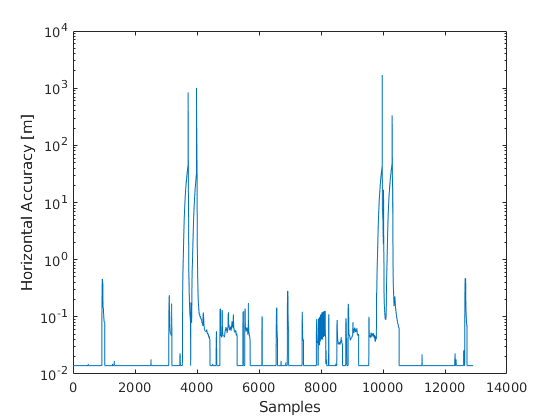
\includegraphics[width=0.7\textwidth]{images/RTKAccDrv}
	\caption{The estimated accuracy by the u-blox module during a ride. The most remote spot was 8\;km away from the HSR. The measurement was sampled with 10\;Hz.}
	\label{fig:rtkhf}
\end{figure}

\begin{figure}[htb]
	\centering
	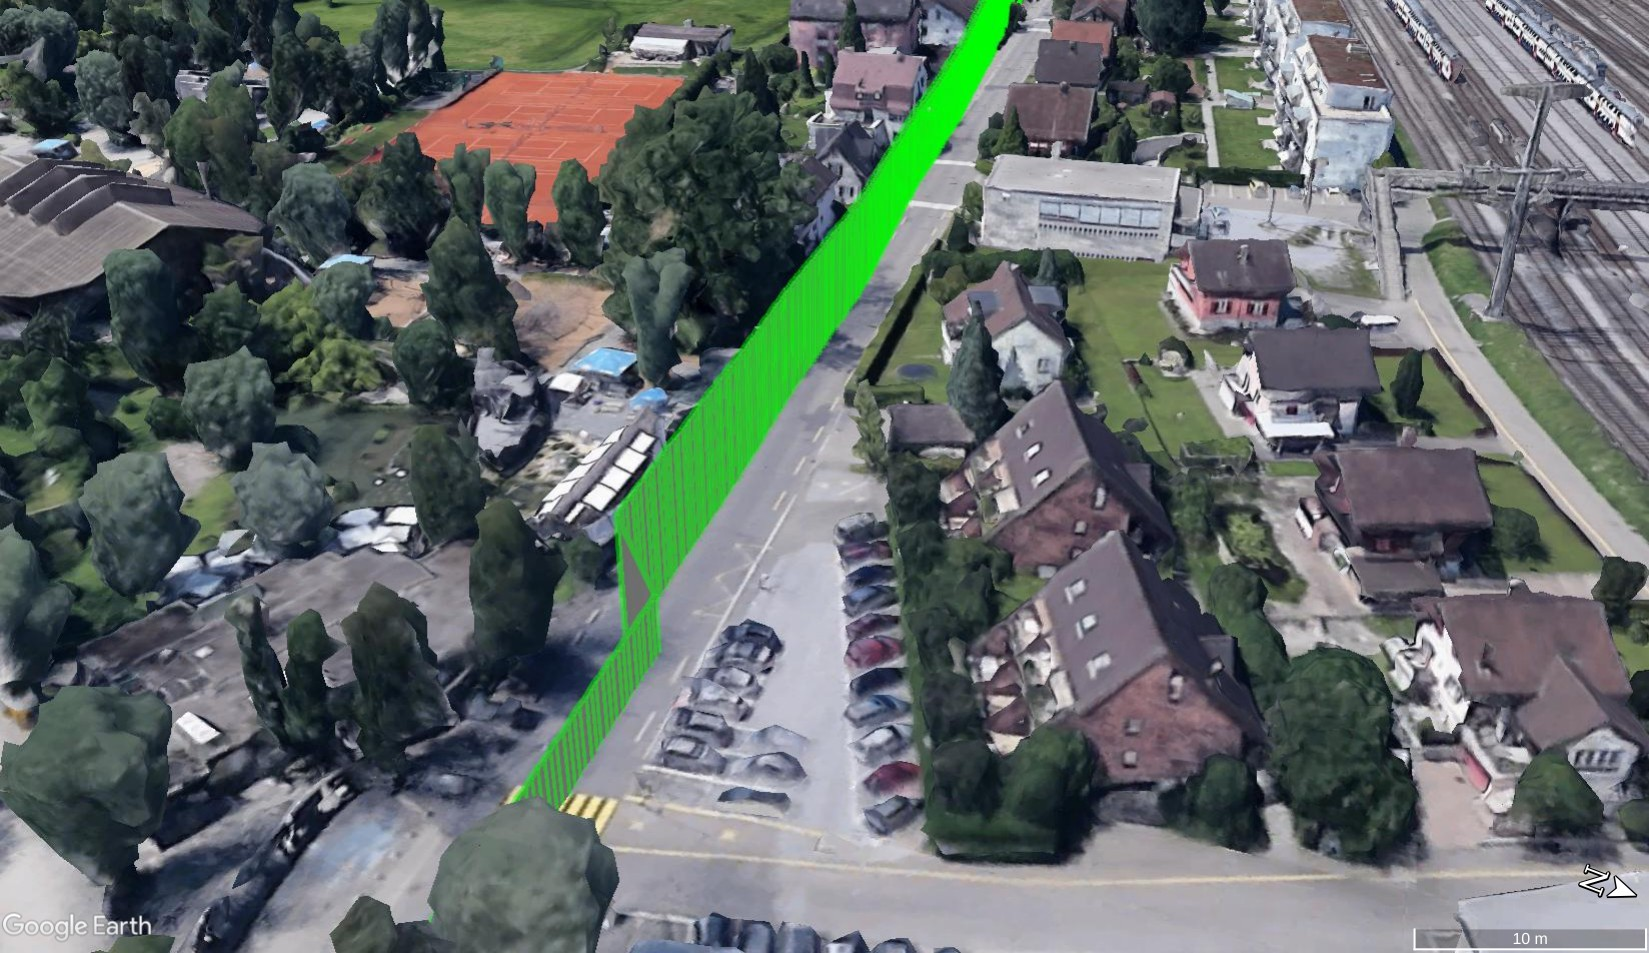
\includegraphics[width=0.7\textwidth]{images/RTK_Messfahrt_fix}
	\caption{Start receiving RTCM data while driving}
	\label{fig:RTKMFfix}
\end{figure}

\begin{figure}[htb]
	\centering
	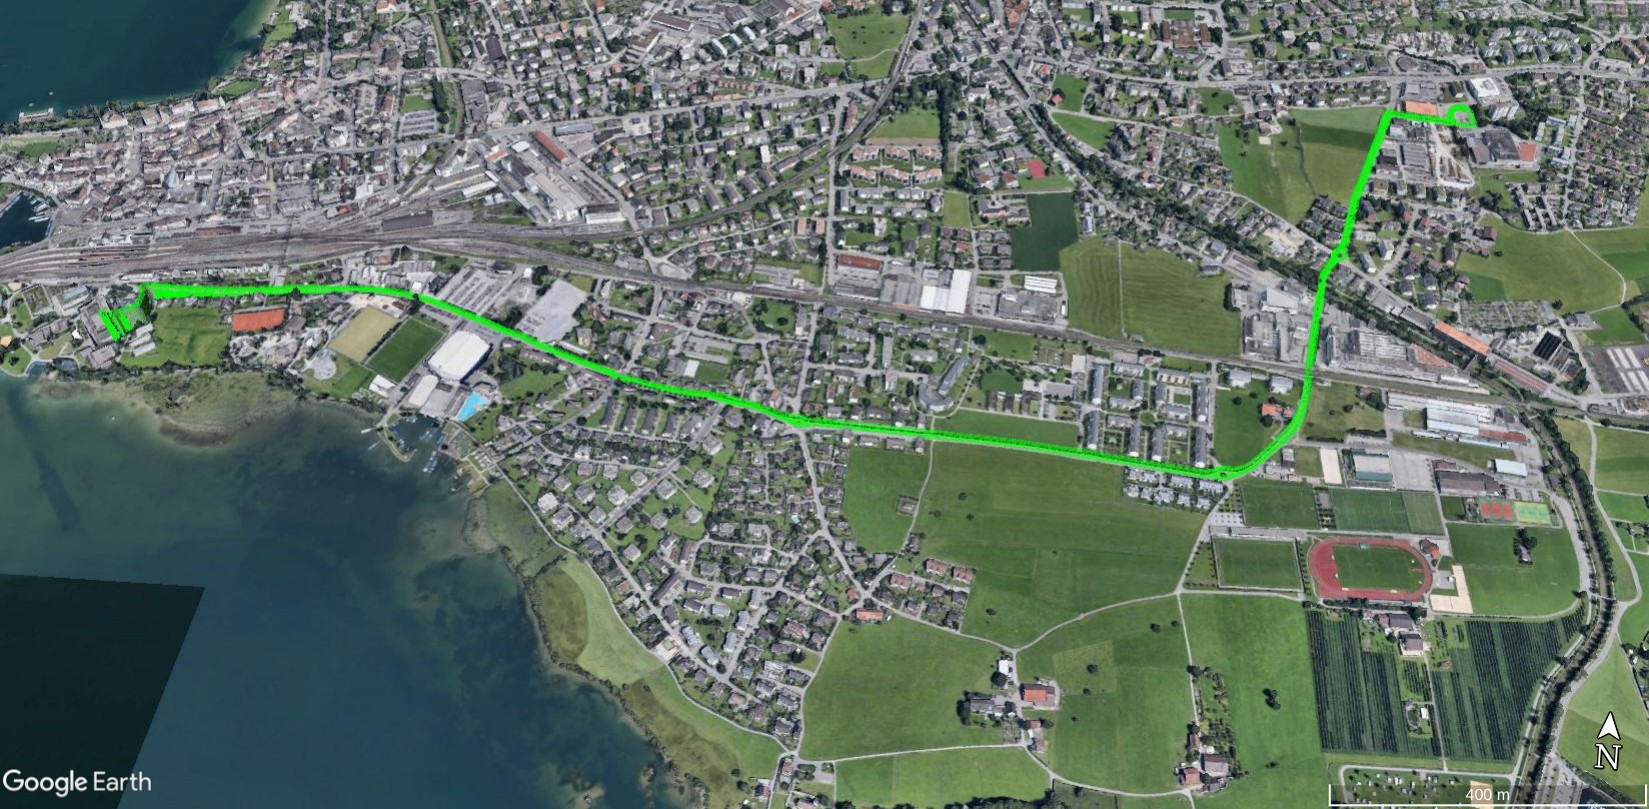
\includegraphics[width=0.7\textwidth]{images/RTK_Messfahrt}
	\caption{Driving with RTK}
	\label{fig:RTKMF}
\end{figure}

\clearpage
\pagebreak
